\documentclass{classrep}
\usepackage[utf8]{inputenc}
\usepackage[pdftex]{graphicx}
\usepackage[polish]{babel}
\usepackage{algorithm}
\usepackage{algorithmic}
\usepackage{multicol}
\usepackage{amsmath}
\usepackage{listings}
\usepackage{array}
\usepackage{multirow}
\usepackage{url}
\usepackage{subfigure}

\studycycle{Informatyka, studia dzienne, II st.}
\coursesemester{I}

\coursename{Przetwarzanie obrazów i dźwięków}
\courseyear{2010/2011}

\courseteacher{xxxxxx}
\coursegroup{xxxxxx}
\svnurl{xxxxxx}

\author{%
  \studentinfo{Michał Janiszewski}{169485} \and
  \studentinfo{Michał Kawski}{xxxxxx}
}

\title{Zadanie 1: Przetwarzanie obrazów}

\floatname{algorithm}{Algorytm}

\usepackage{wasysym}

\begin{document}

\maketitle

\section{Cel zadania}
Celem zadania było stworzenie szkieletu aplikacji do przetwarzania i analizy obrazów i dźwięków oraz zaimplementowanie następujących operacji dotyczących przetwarzania obrazu:
\begin{itemize}
 \item operacje podstawowe:
  \begin{itemize}
   \item zmiana kontrastu obrazu,
   \item zmiana jasności obrazu,
   \item wyznaczanie negatywu obrazu,
  \end{itemize}
 \item filtrowanie obrazu w oparciu o:
  \begin{itemize}
   \item filtr ze średnią arytmetyczną,
   \item filtr medianowy,
  \end{itemize}
 \item wyznaczanie i pokazywanie histogramu obrazu dla poszczególnych jego kanałów, a także umożliwienie edycji obrazu na podstawie tego histogramu,
 \item filtracja liniowa oparta o splot z możliwością zdefiniowania rozmiaru i wartości maski,
 \item filtracja nieliniowa w dziedzinie czasu.
\end{itemize}

Wylosowane warianty zadań to:
\begin{itemize}
 \item histogramy H3 \ppauza wyjściowa gęstość prawdopodobieństwa podana wzorem Raleigha:
  \begin{equation*}
   g(f) = g_{min} + \left(2 \alpha^2 \ln \left(\frac{1}{N} \displaystyle\sum\limits_{m=0}^f H\left(m\right)\right)^{-1}\right)^{\frac{1}{2}}
  \end{equation*}
 \item splot S4 \ppauza wydobywanie szczegółów z tła: południe, południowy-zachód, zachód, północny-zachód:
\begin{equation*}
\left(\begin{array}{ccc} -1 & -1 & -1 \\ 
1 & -2 & 1 \\
1 & 1 & 1 \\
\end{array}\right)\\
\\
\left(\begin{array}{ccc} 1 & -1 & -1 \\ 
1 & -2 & -1 \\
1 & 1 & 1 \\
\end{array}\right)\\
\\
\left(\begin{array}{ccc} 1 & 1 & -1 \\ 
1 & -2 & -1 \\
1 & 1 & -1 \\
\end{array}\right)\\
\\
\left(\begin{array}{ccc} 1 & 1 & 1 \\ 
1 & -2 & -1 \\
1 & -1 & -1 \\
\end{array}\right)
\end{equation*}
  \item filtracja nieliniowa O5 \ppauza operator Rosenfelda:
\begin{equation*}
 g(x, y) = \frac{1}{R} \left( \displaystyle \sum \limits_{i=1}^R f\left(x + i - 1, y\right) - \displaystyle \sum \limits_{i=1}^R f \left(x - i, y\right) \right)
\end{equation*}
\end{itemize}

\section{Opis metod przetwarzania}

Poniżej znajduje się opis algorytmów realizujących opisane powyżej zagadnienia. Obsługiwane są 3 typy obrazów:
\begin{enumerate}
 \item obrazy kolorowe (24-bitowe),
 \item obrazy w 8-bitowej skali szarości,
 \item obrazy binarne (1-bitowe).
\end{enumerate}

W przypadku obrazu kolorowego zakładamy, że każdy piksel ma trzy kanały: R (czerwony), G (zielony) i B (niebieski), a wartość każdego z tych pikseli znajduje się w zakresie $[0; 255]$ i przyjmuje tylko wartości całkowite.

W przypadku obrazów w skali szarości przyjmujemy, że każdy piksel posiada tylko jedną, 8-bitową składową, jest to indeks koloru z palety barw zapisanej w obrazie. Chociaż możliwe jest zapisanie dowolnej palety kolorów, przyjmujemy, że mamy do czynienia tylko i wyłącznie z obrazami w skali szarości (lub innego koloru), a 256 dostępnych, unikatowych kolorów w palecie uporządkowanych jest od najjaśniejszego (białego) do najbardziej intensywnego (czarnego \ppauza w przypadku skali szarości).

Piksele w obrazach binarnych przyjmują tylko dwa dostępne stany: biały i czarny.

Ponadto, przyjmijmy następujące oznaczenia:
\begin{description}
 \item[$g(n, m)$] wartość kanału piksela o współrzędnych $(n, m)$,
 \item[$g'(n, m)$] piksel o współrzędnych $(n, m)$ w obrazie wyjściowym,
 \item[$N, M$] odpowiednio szerokość i wysokość obrazu w pikselach.
\end{description}


\subsection{Operacje podstawowe}

Opisane poniżej operacje podstawowe ograniczają swoje działanie tylko do jednego piksela, tzn. wartość funkcji przekształcenia nie zależy od otoczenia w jakim piksel się znajduje.

Algorytmy abstrachują od szczegółów implementacji, dzięki czemu można opisać ich działanie dla wszystkich wymienionych wyżej typów obrazów.

Ponieważ piksele w operacjach tych przetwarzane są niezależnie, przetwarzanie obrazu za ich pomocą sprowadza się do przetworzenia każdego piksela obrazu zadanym algorytmem.

\subsubsection{Negatyw}
\label{filter.negative}
Wyznaczanie negatywu obrazu sprowadza się do wyznacznia wartości przeciwnej dla każdego z kanałów piksela:

\begin{equation}
 g'(n, m) = -g(n, m) \mod C_{max}
\end{equation}

gdzie $C_{max}$ to maksymalna możliwa wartość.

\subsubsection{Zmiana kontrastu}
\label{filter.contrast}
Zmiana kontrastu to zmiana amplitudy charakteryzującej każdy z kanałów piksela. Dokonujemy tego poprzez mnożenie wartości każdego z kanałów przez pewien współczynnik $\alpha \in [0; 2]$, a następnie ograniczamy tak uzyskane wartości do zakresu możliwych:
\begin{equation}
\label{eq.contrast}
 f(n, m) = g(n, m) \cdot \alpha
\end{equation}
\begin{equation}
 g'(n, m) = \left\{
  \begin{array}{l l}
    0 & \quad f(n, m) < 0 \\
    f(n, m) & \quad 0 \leq f(n, m) \leq C_{max} \\
    C_{max} & \quad f(n, m) > C_{max} \\
  \end{array}
\right.
\end{equation}

\subsubsection{Zmiana jasności}
\label{filter.brightness}
Zmiana jasności sprowadza się do dodania pewnej stałej $\delta$ do każdego kanału piksela. $\delta$ może przyjmować wartości zarówno dodatnie jak i ujemne, co określa odpowiednio rozjaśnianie oraz przyciemnianie obrazu. Tak przetworzone wartości należy ograniczyć jeszcze do wartości możliwych do zapisania w obrazie:
\begin{equation}
\label{eq.brightness}
 f(n, m) = g(n, m) + \delta
\end{equation}
\begin{equation}
 g'(n, m) = \left\{
  \begin{array}{l l}
    0 & \quad f(n, m) < 0 \\
    f(n, m) & \quad 0 \leq f(n, m) \leq C_{max} \\
    C_{max} & \quad f(n, m) > C_{max} \\
  \end{array}
\right.
\end{equation}

\subsection{Filtrowanie}
Filtrowanie obrazu jest próbą poprawienia jego jakości \ppauza zarówno obiektywnej jak i subiektywnej. Zadaniem zaimplementowanych filtrów jest usuwanie szumów z obrazu.

Każdy z tych filtrów, w odróżnieniu od operacji podstawowych, uwzględnia okolicę piksela, do której należy przetwarzany aktualnie piksel. Wielkość otoczenia nazywana jest wielkością maski i określa, ile pikseli zarówno w poziomie jak i pionie branych jest pod uwagę podczas wyliczania nowej wartości przetwarzanego piksela.

W przypadku gdy maska określa pobranie wartości piksela spoza obrazka, element taki zostaje zignorowany i nie jest brany pod uwagę w obliczeniach.

\subsubsection{Filtr ze średnią arytmetyczną}
\label{filter.average}
Dla każdego kanału piksela obrazu sumowane są wartości tego kanału z wszystkich pikseli odległych od aktualnie przetwarzanego nie więcej, niż określa to rozmiar maski. Suma ta jest następnie dzielona przez ilość uwzględnionych elementów \ppauza obliczana jest średnia arytmetyczna:
\begin{equation}
 g'(n, m) = \frac{1}{(2 \cdot w + 1) \cdot (2 \cdot h + 1)} \cdot \displaystyle \sum \limits_{n' = n - w}^{n + w} \displaystyle \sum \limits_{m' = m - h}^{m + h} g(n', m')
\end{equation}
gdzie $w$ to promień poziomy, a $h$ promień pionowy maski.

\subsubsection{Filtr medianowy}
\label{filter.median}
W przypadku filtru medianowego wartości kanału ze wszystkich pikseli wchodzących w skład maski ustawiane są w niemalejącym szeregu, a następnie zwracana jest mediana tych elementów, czyli element z pozycji $\frac{l}{2}$~w~przypadku szeregu o nieparzystej długości $l$ lub średnia arytmetyczna z~dwóch środkowych elementów $\frac{g(\frac{l}{2} - 1) + g(\frac{l}{2})}{2}$ w przypadku szeregu o parzystej ilości elementów.

\subsection{Modyfikacja w oparciu o histogram}

\subsection{Filtracja liniowa w oparciu o splot}
\label{filter.convolution}
Aby dokonać filtracji liniowej opartej o splot, konieczna jest znajomość maski filtru, jaka opisuje odpowiedź impulsową splotu. Nazwijmy tę maskę macierzą $X[2 \cdot W + 1; 2 \cdot H + 1]$ i przyjmijmy, że funkcja $x(w, h)$ zwraca element macierzy $X$ z pozycji $(w, h)$, wtedy:
\begin{equation}
 g'(n, m) = \displaystyle \sum \limits_{w=-W}^W \displaystyle \sum \limits_{h=-H}^H g(n + w, m + h) \cdot x(w, h)
\end{equation}

Uzyskane w taki sposób wartości należy znormalizować. W tym celu postanowiliśmy znaleźć minimalną i maksymalną wartość kanału $C'_{min}$ oraz $C'_{max}$ po przekształceniu, a następnie przeskalować wszystkie wartości z tego zakresu na zakres możliwy do osiągnięcia $C_{min} \div C_{max}$\footnote{Wartość $C_{min}$ wynosi 0, zatem można ją pominąć w obliczeniach}:
\begin{equation}
 \label{eq:normalization}
 c = \frac{C_{max}}{C'_{max} - C'_{min}} \cdot (c' - C'_{min})
\end{equation}

\subsection{Filtracja nieliniowa}
\label{filter.nonlinear}
Wariant zadania, który nam przypadł przewidywał implementację poziomego operatora Rosenfelda:
\begin{equation}
 g'(n, m) = \frac{1}{R} \cdot \left( \displaystyle \sum \limits_{i=1}^R g\left(n + i - 1, m\right) - \displaystyle \sum \limits_{i=1}^R g\left(n - i, m\right) \right)
\end{equation}
Normalizacja uzyskanych danych ma postać jak w równaniu \ref{eq:normalization}.

\subsection{Obiektywna ocena jakości obrazu}
Ponieważ do każdego z zaszumionych obrazów testowych dostępne są wersje oryginalne, o idealnej jakości, można dokonać obiektywnej oceny jakości filtrowania. Zaimplementowane metody porównują odstępstwa przetworzonego obrazu zaszumionego z obrazem oryginalnym.

\subsubsection{MSE}
MSE, czyli \textit{Mean Square Error}, błąd średniokwadratowy $E$, jest podstawowym kryterium pomiarowym. Zlicza on sumę kwadratów różnic pomiędzy wartościami otrzymanymi, a idealnymi:
\begin{equation}
 E = \frac{1}{N \cdot M} \displaystyle \sum \limits_{n=0}^{N-1} \sum \limits_{m=0}^{M-1} \left(g\left(n, m\right) - g'\left(n, m\right) \right)^2
\end{equation}
W tym przypadku $g'$ odnosi się do przefiltrowanego obrazu.

\subsubsection{SNR}
SNR, czyli \textit{Signal to Noise Ratio}, współczynnik sygnału do szumu $R$, stanowi często spotykaną metodę określania jakości sygnału. Wyznaczany jest wzorem:
\begin{equation}
 R = 10 \log_{10} \frac{\displaystyle \sum \limits_{n=0}^{N-1} \sum \limits_{m=0}^{M-1} \left(g\left(n, m\right)\right)^2}{E}
\end{equation}
$E$ to wyznaczony powyżej współczynnik MSE.

\section{Implementacja}
Program powstał przy wykorzystaniu frameworku Qt wykorzystującego język C++.

Po uruchomieniu programu prezentowane jest użytkownikowi okienko klasy \texttt{MainWindow}. Umożliwia ono wybranie pliku z obrazem do otwarcia. Użytkownik może wybrać dowolny format wspierany przez bibliotekę Qt, a dzięki możliwości pisania wtyczek \ppauza zakres ten można powiększać.

Po wybraniu pliku obrazu do otwarcia, tworzona jest nowa instancja klasy \texttt{PhotoWindow}. W konstruktorze ładuje on podany jako argument plik, ustawia go jako prezentowany za pomocą kontrolki klasy \texttt{QLabel} obrazek oraz inicjalizuje filtry.

Każdy z filtrów dziedziczy po interfejsie \texttt{FilterInterface} skonstruowanym za pomocą klasy wirtualnej. Część metod tej klasy jest zaimplementowana \ppauza dostarczają one środków do identyfikacji filtrów. Do implementacji w klasie pochodnej pozostawione zostały metody:
\begin{itemize}
 \item \texttt{virtual QString name() const} \ppauza zwracająca nazwę filtru,
 \item \texttt{virtual QImage apply()} \ppauza uruchamiająca działanie filtru.
\end{itemize}

Ponadto filtry powinny też dostarczać implementacji metody \texttt{virtual bool setup(const QImage \&)} w której inicjalizowane są parametry filtru. Podejście takie pozwala sprawdzić, czy użytkownik zatwierdził wykonanie operacji oraz czy wprowadzone parametry są poprawne. Dopiero po tych testach może zostać zwrócona wartość \texttt{true}, która komunikuje gotowość do uruchomienia filtra.

Z menu użytkownik może wybrać także opcję zapisania obrazka \ppauza obrazek zapisywany jest w formacie PNG, pokazania lub ukrycia okna histogramów, uruchomienia wspomnianych filtrów oraz sprawdzenia jakości obrazka.

W tym ostatnim przypadku należy załadować do programu zaszumiony obrazek i poddać go litracji, po kliknięciu wspomnianej opcji pojawi się okienko, w którym użytkownik powinien wskazać położenie pliku oryginalnego, zaś parametry MSE i SNR zostaną wypisane na wyjście błędów.

Uruchomienie filtru na obrazku skutkuje utworzeniem nowego okna klasy \texttt{PhotoWindow} wyświetlającym przetworzony obrazek. Tak wyświetlone okno w swoim tytule pokazuje, jakie operacje były wykonane na obrazku.

\subsection{Filtry}
Wszystkie filtry, w tym splot oraz filtracja nieliniowa opierają się o klasę \texttt{FilterInterface}. Instancje klas dziedziczących po niej tworzone są w konstruktorze \texttt{PhotoWindow} i wypełniane jest nimi submenu Filters. Wywołanie jednej z dostępnych opcji skutkuje wywołaniem metody \texttt{setup()}, a jeśli zwróci ona wartość true, wykonywana jest także metoda \texttt{apply}, która zwraca przetworzony obrazek.

\subsubsection{Negatyw - Negative}
Filtr ten nie posiada opcji, wykonuje metodę opisaną w sekcji \ref{filter.negative}.

\subsubsection{Jasność - Brightness}
Po wybraniu tego filtru prezentowane jest użytkownikowi okienko, w którym określany jest parametr $\delta$ opisany w sekcji \ref{filter.brightness}, a następnie metoda z tej sekcji wykonywana jest dla całego obrazu.

\subsubsection{Kontrast - Contrast}
Wybranie tego filtru skutkuje prezentacją użytkownikowi okienka z suwakiem służącym do wyboru pożądanej wielkości parametru $\alpha$ z sekcji \ref{filter.contrast}. Możliwe jest wybranie wartości z zakresu $-255 \div 255$, wybrana wartość jest następnie dzielona przez 255 i dodawana do 1, aby przeskalować ją na zakres $[0; 2]$.

\subsubsection{Uśrednianie - Average}
Uruchomienie tego filtru powoduje pokazanie okienka z wyborem wielkości maski \ppauza użytkownik powinien wprowadzić promień poziommy i pionowy maski, po czym następuje wykonanie metody opisanej w \ref{filter.average}.

\subsubsection{Mediana - Median}
Włączenie tego filtru spowoduje działanie podobne jak w powyższym przypadku \ppauza ukazanie się okienka z wyborem maski, a następnie zostanie wykonana metoda z sekcji \ref{filter.median}.

\subsubsection{Filtr liniowy - Convolution}
Wybranie tej opcji spowoduje najpierw pokazanie okienka z wyborem wielkości maski, następnie zaś użytkownik zostanie poproszony o wprowadzenie wartości maski. Metoda ta jest opisana w sekcji \ref{filter.convolution}.

\subsubsection{Filtr nieliniowy - Rosenfeld}
Opcja ta spowoduje pokazanie okienka z suwakiem, w którym użytkownik powinien podać parametr $R$.

\section{Materiały i metody}
Do testów wykorzystaliśmy popularny obrazek ,,Lena'' w wariantach kolorowym i odcieni szarości. Obrazki te prezentują rysunki \ref{fig.lena} i \ref{fig.lenac}.

\begin{figure}
  \begin{minipage}{0.5\linewidth}
    \centering
    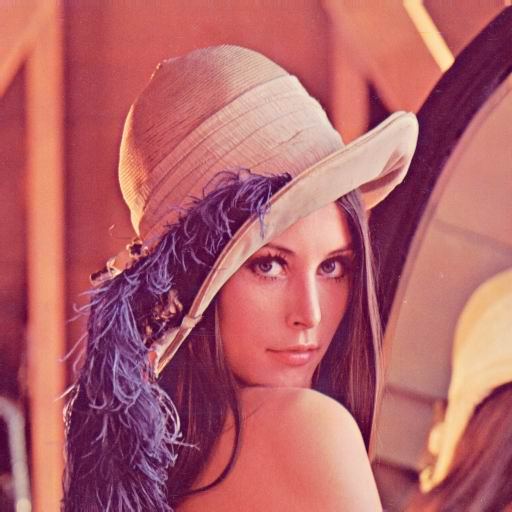
\includegraphics[scale=0.4]{img/lenac.png}
    \caption{Obraz kolorowy \textbf{lenac.bmp} wykorzystany do testów.}
    \label{fig.lena}
  \end{minipage}
  \hspace{0.5cm}
  \begin{minipage}{0.5\linewidth}
    \centering
    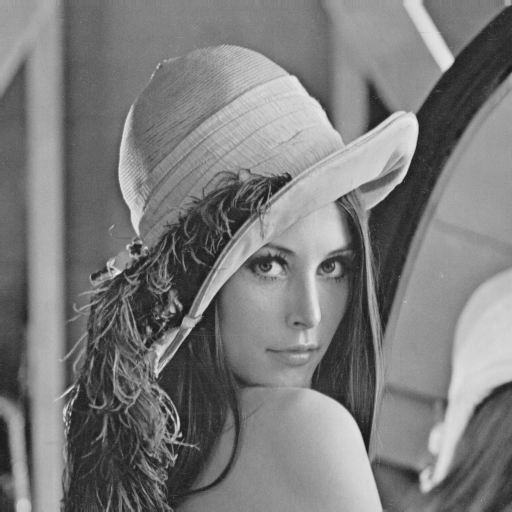
\includegraphics[scale=0.4]{img/lena.png}
    \caption{Obraz czarno-biały \textbf{lena.bmp} wykorzystany do testów.}
    \label{fig.lenac}
  \end{minipage}
\end{figure}

\begin{figure}
\noindent\makebox[\textwidth]{%
 \subfigure[Obraz kolorowy z szumem o rozkładzie normalnym \textbf{lenac\_normal3.bmp} wykorzystany do testów.]{
  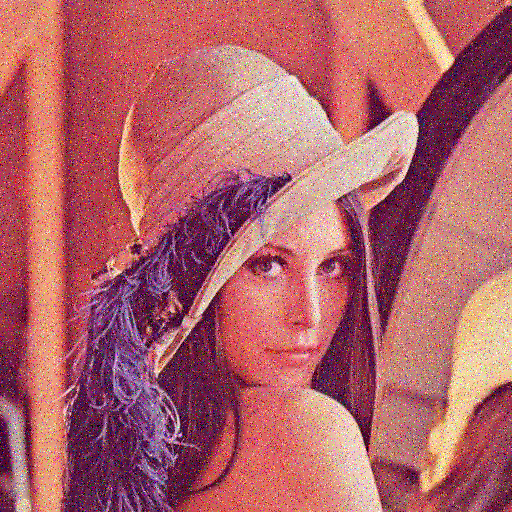
\includegraphics[scale=0.3]{img/lenac_normal3.png}
  \label{fig.lenac_normal3}
 }
 \subfigure[Obraz kolorowy z szumem o rozkładzie jednostajnym \textbf{lenac\_uniform3.bmp} wykorzystany do testów.]{
  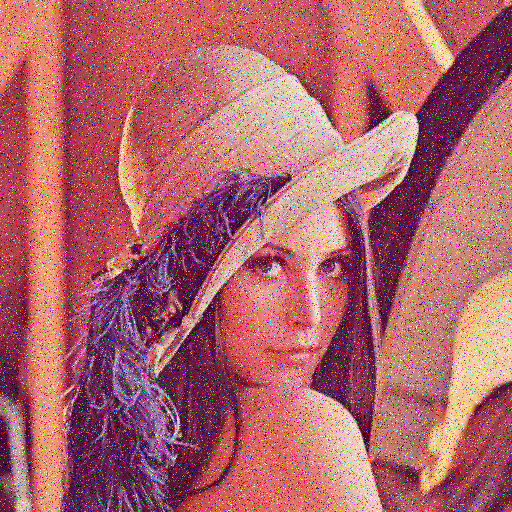
\includegraphics[scale=0.3]{img/lenac_uniform3.png}
  \label{fig.lenac_uniform3}
 }
 \subfigure[Obraz kolorowy z szumem o rozkładzie impulsowym \textbf{lenac\_impulse3.bmp} wykorzystany do testów.]{
  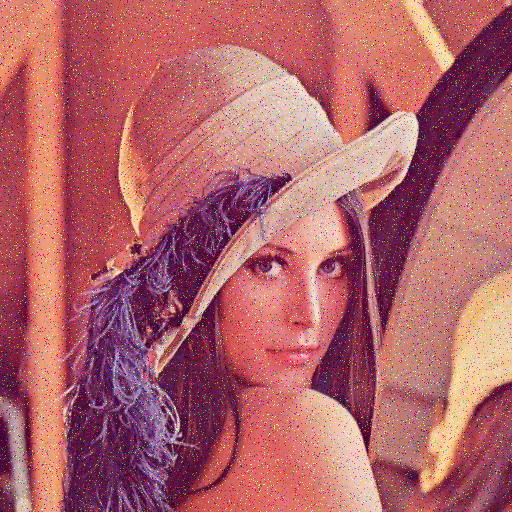
\includegraphics[scale=0.3]{img/lenac_impulse3.png}
  \label{fig.lenac_impulse3}
 }
}
\caption{Zaszumione kolorowe obrazy}
\end{figure}

\begin{figure}
\noindent\makebox[\textwidth]{%
 \subfigure[Obraz w skali szarości z szumem o rozkładzie normalnym \textbf{lena\_normal3.bmp} wykorzystany do testów.]{
  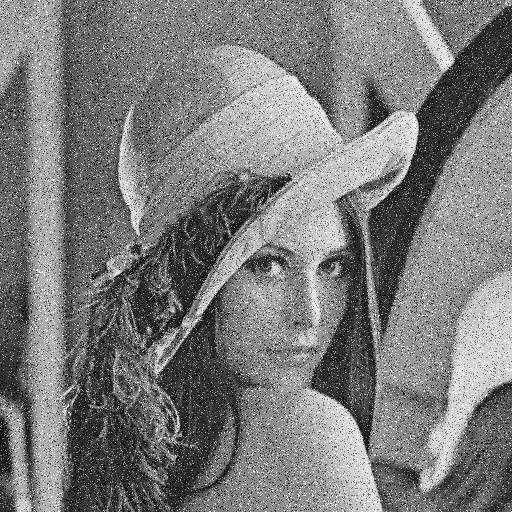
\includegraphics[scale=0.3]{img/lena_normal3.png}
  \label{fig.lena_normal3}
 }
 \subfigure[Obraz w skali szarości z szumem o rozkładzie jednostajnym \textbf{lena\_uniform3.bmp} wykorzystany do testów.]{
  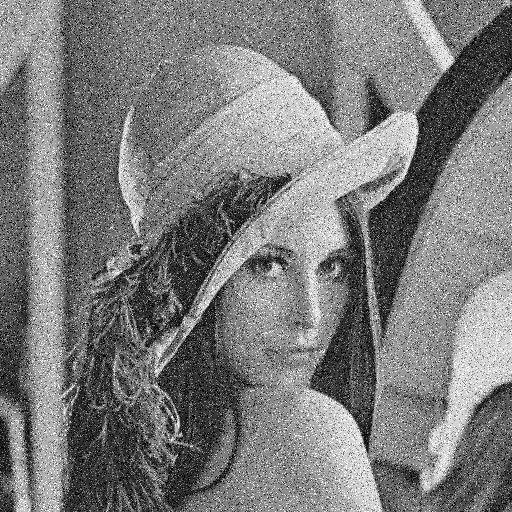
\includegraphics[scale=0.3]{img/lena_uniform3.png}
  \label{fig.lena_uniform3}
 }
 \subfigure[Obraz w skali szarości z szumem o rozkładzie impulsowym \textbf{lena\_impulse3.bmp} wykorzystany do testów.]{
  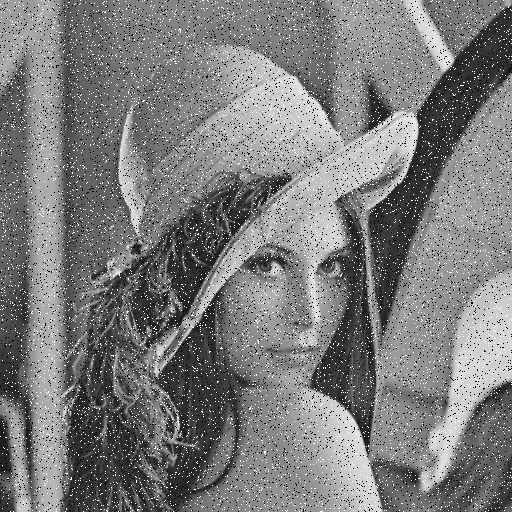
\includegraphics[scale=0.3]{img/lena_impulse3.png}
  \label{fig.lena_impulse3}
 }
}
\caption{Zaszumione obrazy w skali szarości}
\end{figure}

Ponadto dla każdego wariantu wybraliśmy trzy rodzaje szumów:
\begin{itemize}
 \item szum o rozkładzie normalnym (rysunki \ref{fig.lenac_normal3} i \ref{fig.lena_normal3}),
 \item szum o rozkładzie jednostajnym (rysunki \ref{fig.lenac_uniform3} i \ref{fig.lena_uniform3}),
 \item szum o rozkładzie impulsowym (rysunki \ref{fig.lenac_impulse3} i \ref{fig.lena_impulse3}).
\end{itemize}

Podstawowe wersje rysunków zostały poddane działaniu wszystkich filtrów, zaś obrazy zaszumione tylko filtrowaniu z wykorzystaniem średniej i mediany.

Poniżej znajdują się opisane szczegółowo działania.

\subsection{Negatyw}
Wyznaczony został negatyw obrazków za pomocą filtru Negative.

\subsection{Zmiana jasności}
Dokonano zmiany jasności obrazków za pomocą filtru Brightness. Obrazki przyciemniono oraz rozjaśniono stosując wartość parametru wynoszącą odpowiednio -85 oraz +85, co odpowiada wartościom $-\frac{1}{3}$ oraz $\frac{1}{3}$ parametru $\delta$ ze wzoru \ref{eq.brightness}.

\subsection{Zmiana kontrastu}
Dokonano zmiany kontrastu obrazków za pomocą filtru Contrast. Obrazkom zwiększono i zmniejszono kontrast stosując do tego następujące parametry: -85 oraz +85, co odpowiada wartościom $-\frac{1}{3}$ oraz $\frac{1}{3}$ parametru $\alpha$ ze wzoru \ref{eq.contrast}.

\subsection{Filtrowanie}
\subsubsection{Za pomocą średniej arytmetycznej}
Dokonano trzech filtrowań, z maskami o wielkościach $3 \times 3$, $5 \times 5$, $7 \times 7$ za pomocą filtru Average. Filtrowaniu poddane zostały obrazki oryginalne oraz zaszumione.

\subsubsection{Za pomocą mediany}
Dokonano trzech filtrowań, z maskami o wielkościach $3 \times 3$, $5 \times 5$, $7 \times 7$ za pomocą filtru Median. Filtrowaniu poddane zostały obrazki oryginalne oraz zaszumione.

\subsection{Modyfikacja w oparciu o histogram}

\subsection{Filtracja liniowa w oparciu o splot}
Dokonano filtracji liniowej opartej o splot. Przydzielony wariant zadania określał wykorzystanie następujących masek: wydobywanie szczegółów z tła: południe, południowy-zachód, zachód, północny-zachód:
\begin{equation*}
\left(\begin{array}{ccc} -1 & -1 & -1 \\ 
1 & -2 & 1 \\
1 & 1 & 1 \\
\end{array}\right)\\
\\
\left(\begin{array}{ccc} 1 & -1 & -1 \\ 
1 & -2 & -1 \\
1 & 1 & 1 \\
\end{array}\right)\\
\\
\left(\begin{array}{ccc} 1 & 1 & -1 \\ 
1 & -2 & -1 \\
1 & 1 & -1 \\
\end{array}\right)\\
\\
\left(\begin{array}{ccc} 1 & 1 & 1 \\ 
1 & -2 & -1 \\
1 & -1 & -1 \\
\end{array}\right)
\end{equation*}

\subsection{Filtracja nieliniowa}
Dokonano filtracji nieliniowej obrazu wykorzystując w tym celu operator Rosenfelda z następującymi parametrami R: 2, 3, 4, 5, 6.

\subsection{Obiektywna i subiektywna ocena jakości obrazu}
Przefiltrowane zaszumione wersje obrazów poddano ocenie. W celu obiektywnej oceny jakości wykorzystano wskaźniki MSE i SNR, natomiast do oceny subiektywnej wykorzystano własne oczy \smiley.

\begin{thebibliography}{99}
%\bibitem{pleple}
% opis
\end{thebibliography}

\end{document}
